\documentclass[11pt]{article}
\usepackage[spanish,es-noshorthands]{babel}
\usepackage[utf8]{inputenc}
\usepackage[T1]{fontenc}
\usepackage[margin=2cm]{geometry}
\usepackage{graphicx,booktabs,array,amsmath,hyperref}
\usepackage[backend=biber,style=apa,natbib=true]{biblatex}
\addbibresource{referencias.bib}
\hypersetup{colorlinks=true,linkcolor=black,citecolor=black,urlcolor=blue}
\title{Proyecto integrador: detección de neumonía en radiografías de tórax\\\large Segunda entrega --- Fase 2: replicación y traslado}
\author{Francy Umbarila \and Juan Delgado \and Andrés Escobar}
\date{Bogotá, D. C. --- septiembre de 2026}
\begin{document}
\maketitle
\section{Objetivo y protocolo congelado}
Se realiza una \emph{replicación reducida} y trazable del enfoque de transferencia de \textcite{rahman2020} para clasificación binaria por imagen: neumonía ($1$) frente a sin hallazgos ($0$). El desarrollo inicial usa Kermany, radiografías pediátricas de Guangzhou \parencite{kermany2018}; el protocolo de traslado reserva una partición de BRAX, radiografías de adultos brasileños \parencite{reis2022a}, para adaptación y prueba externa aislada. La métrica decisoria es sensibilidad de neumonía con especificidad mínima de 0,80 fijada en validación. AUC-ROC, AUPRC, F1, matrices de confusión, latencia e intervalos bootstrap al 95\% por paciente complementan la evaluación.

El manifiesto contiene \texttt{patient\_id}, \texttt{study\_id}, \texttt{image\_path}, \texttt{view} y \texttt{label}. Se construyó una partición estratificada 70/15/15 por paciente, semilla 42: 4.107/847/902 imágenes y 2.399/514/514 pacientes en entrenamiento/validación/prueba. El código detiene la ejecución ante cualquier paciente compartido. Como limitación de Kermany, los identificadores de pacientes normales se derivan del archivo; este supuesto se conserva y se declara, en vez de reclamar una agrupación clínica que el conjunto no ofrece.

\section{Réplica y transferencia}
La implementación usa PyTorch y DenseNet121 con pesos ImageNet. DenseNet201 era la arquitectura del artículo, pero DenseNet121 reduce el costo de CPU y memoria; por ello esta no es una réplica numérica ni arquitectónica exacta. Rahman et al. emplearon MATLAB, SGD, otra partición y validación cruzada. La entrada es $224\times224$, la radiografía gris se convierte a RGB y se normaliza con estadísticas ImageNet. Solo entrenamiento recibe afín aleatoria ($\pm10^\circ$, traslación y escala de 5\%); no hay aumento en validación, prueba ni prueba externa BRAX.

\begin{table}[h]\centering\small
\caption{Contraste honesto de la tarea binaria con el artículo. No es una comparación causal: cambian arquitectura, número de imágenes, partición y protocolo.}\label{tab:replica}
\begin{tabular}{lccc}\toprule
Fuente/configuración & Sensibilidad & Especificidad & F1 \\\midrule
Rahman et al.: DenseNet201 & 0,990 & 0,970 & 0,981\\
Esta entrega: DenseNet121, ajuste parcial (media de tres semillas) & 0,992 & 0,869 & 0,973\\\bottomrule
\end{tabular}
\end{table}

Se reproduce el flujo central ---CNN preentrenada, ajuste por transferencia y clasificación normal/neumonía--- y se obtiene una sensibilidad de orden comparable. No se reproduce el resultado publicado de forma exacta: además de la sustitución DenseNet201$\rightarrow$DenseNet121, el artículo reporta 5.247 imágenes mientras este manifiesto contiene 5.856 y la evaluación aquí es una única partición 70/15/15 por paciente. La menor especificidad observada y cualquier diferencia de F1 se interpretan bajo esas diferencias, no como contradicción del artículo.

\begin{table}[h]\centering\small
\caption{Configuración reproducible de Fase 2.}\label{tab:config}
\begin{tabular}{ll}\toprule
Elemento & Decisión \\\midrule
Arquitectura/pesos & DenseNet121 / ImageNet (reducción de DenseNet201 por cómputo)\\
Pérdida/optimizador & BCE ponderada / Adam con $10^{-4}$ en clasificador\\
Transferencia A & Extractor congelado; solo clasificador final\\
Transferencia B & Clasificador y \texttt{denseblock4}; $10^{-5}$ en bloque ajustado\\
Selección & AUC de validación, ReduceLROnPlateau y parada temprana (paciencia 5)\\
Semillas & 42, 43 y 44; seis corridas ejecutadas\\
Umbral & Máxima sensibilidad con especificidad $\geq0,80$, solo validación\\\bottomrule
\end{tabular}
\end{table}

\section{Dinámica y evaluación interna}
Cada corrida guarda configuración, historial por época (pérdida, AUC de entrenamiento y validación, tasa de aprendizaje, norma media de gradiente y duración), checkpoint y predicciones con IDs. El checkpoint de AUC de validación máxima se recarga antes de fijar el umbral y evaluar una única vez el test. Así, la norma de gradiente se mide: cualquier diagnóstico de explosión o desaparición se sustenta en esa serie, no en una inferencia visual. En las seis corridas la norma media permaneció dentro de la banda $[1{,}05;\ 1{,}92]$, con tendencia descendente pero no monótona, sin picos ni acercamiento a cero: no hay evidencia de explosión ni de desaparición de gradiente.

El \texttt{train\_auc} del historial se acumula con los logits producidos durante la propia época, sobre imágenes aumentadas y con los pesos cambiando entre lotes. No equivale a una pasada de evaluación limpia posterior al entrenamiento y tiende a subestimar el desempeño real sobre entrenamiento; se adoptó esta definición para no recorrer la partición de entrenamiento por segunda vez en cada época. El \texttt{val\_auc}, que es la métrica de selección, sí proviene de una pasada de evaluación sin aumento.

\begin{figure}[h]\centering

\includegraphics[width=\textwidth]{figures/training_curves.png}
\caption{Curvas generadas automáticamente desde los historiales guardados: pérdida, AUC de entrenamiento/validación, tasa de aprendizaje y norma de gradiente. Los historiales de las seis corridas ya completadas no contienen pérdida de validación; las corridas futuras sí la guardan.}\label{fig:curves}
\end{figure}

\begin{table}[h]\centering\small
\caption{Resultados internos agregados entre semillas. Este archivo se genera solo a partir de \texttt{metrics.json}.}\label{tab:results}
\begin{tabular}{lp{9cm}}\toprule Estado & Evidencia \\ \midrule Pendiente & Ejecute \texttt{make phase2-train}; no se reportan métricas sin una corrida finalizada. \\ \bottomrule\end{tabular}

\end{table}

\begin{figure}[h]\centering
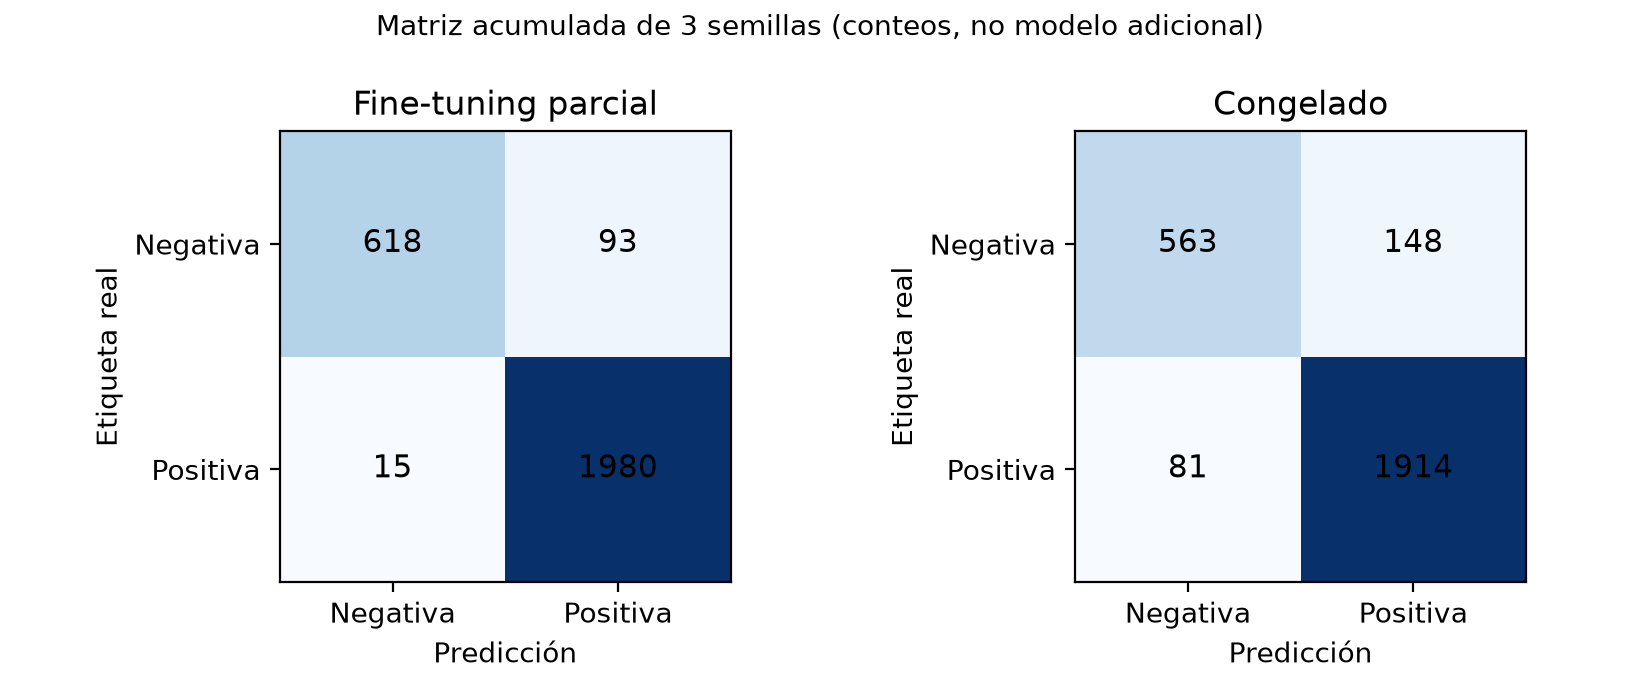
\includegraphics[width=.8\textwidth]{figures/confusion_matrices.png}
\caption{Matrices de confusión agregadas sobre las tres semillas para inspeccionar patrones de FP/FN. Son conteos de corridas, no un séptimo modelo ni una estimación de incertidumbre.}\label{fig:confusion}
\end{figure}

Ambas configuraciones son estables entre semillas: el AUC-ROC varía $\pm0{,}001$ pese a que la época óptima osciló entre 15 y 26. El fine-tuning parcial domina en todas las métricas, con 2.161.153 parámetros entrenables frente a los 1.025 del extractor congelado.

\subsection*{Contraste con el baseline de Fase 1}
El baseline Random Forest se reejecuta sobre la misma partición de prueba: 902 imágenes de 514 pacientes, 665 positivas y 237 negativas, con prevalencia 0,7373 idéntica. Sus predicciones y las de la CNN se emparejan por paciente/estudio; la inferencia se basa en bootstrap pareado de la diferencia, no en el solapamiento de intervalos marginales. El punto del Random Forest, cuyo umbral fue seleccionado solo en validación, alcanza especificidad observada 0,759 en prueba; por tanto su sensibilidad no se rotula como ``sensibilidad con especificidad $\geq0,80$''. Esto corrige la ambigüedad identificada en Fase 1 sin reajustar el umbral con el test.

\begin{table}[h]\centering\small
\caption{Evaluación del criterio de éxito frente a Random Forest.}\label{tab:criterio}
\begin{tabular}{lcc}\toprule
Requisito & Extractor congelado & Fine-tuning parcial \\\midrule
Ventaja de sensibilidad vs. RF & $+2{,}26$ & $\mathbf{+5{,}56}$\\
IC 95\% bootstrap \emph{pareado} de diferencia & $[+0{,}72;\ +4{,}89]$ & $[+3{,}82;\ +7{,}46]$ (semilla 42)\\
Ventaja en las tres semillas & cumple & cumple\\
Latencia por imagen & 13,7 ms & 11,9 ms\\\bottomrule
\end{tabular}
\end{table}

En las semillas 42, 43 y 44, la diferencia pareada CNN parcial menos Random Forest en sensibilidad es $+5{,}56$, $+5{,}71$ y $+5{,}41$ puntos, con IC 95\% $[+3{,}82;\ +7{,}46]$, $[+3{,}97;\ +7{,}53]$ y $[+3{,}61;\ +7{,}31]$, respectivamente. Los tres excluyen cero. En la semilla 42 la diferencia es además $+10{,}55$ de especificidad ($[+3{,}70;\ +17{,}49]$) y $+0{,}049$ de AUC-ROC ($[+0{,}036;\ +0{,}063]$). Así, la evidencia de la ventaja es pareada y consistente entre semillas; no se sustituye con una regla de no solapamiento. El test no se reajusta: se reporta el resultado y la incertidumbre, sin elegir umbrales tras observar prueba.

Queda pendiente el requisito cualitativo del protocolo, la plausibilidad clínica de los mapas Grad-CAM, que corresponde a Fase 3. Hasta entonces no se afirma que la CNN esté justificada, solo que supera los criterios numéricos.

\subsection*{Especificidad por debajo del mínimo en el extractor congelado}
Las tres corridas congeladas quedan bajo la especificidad mínima de 0,80 en test (0,781, 0,797 y 0,797), pese a que el umbral se fijó en validación para satisfacerla. El origen es metodológico: el umbral se elige como el de máxima sensibilidad sujeto a $\mathrm{FPR}\leq0{,}20$, es decir, exactamente en el borde de la restricción. Sin margen, cualquier variación muestral entre validación y test la desplaza, y en esta configuración lo hizo sistemáticamente hacia abajo. Los IC 95\% de especificidad contienen 0,80 en las tres semillas ($[0{,}725;\ 0{,}833]$, $[0{,}748;\ 0{,}847]$ y $[0{,}747;\ 0{,}848]$), de modo que el incumplimiento no es concluyente. El fine-tuning parcial no presenta el problema (0,869 $\pm$ 0,016): al ser más separable, el borde de la restricción deja holgura. No se modificó el criterio de umbral tras observar el test, porque hacerlo contaminaría la selección con información de la partición de prueba.

\section{Traslado a BRAX y limitaciones}
El protocolo BRAX queda definido antes de entrenar. El script filtra adultos PA/AP y clases binarias inequívocas: positivo exige \texttt{Pneumonia=1} y \texttt{No Finding=0}; negativo exige \texttt{Pneumonia=0} y \texttt{No Finding=1}. Así no se equipara mecánicamente ``ausencia de neumonía'' con ``sin hallazgos'' cuando coexisten otros hallazgos. Se excluyen incertidumbres, etiquetas faltantes y combinaciones restantes; el flujo de filtros, prevalencia y tamaños se guarda junto al manifiesto.

Antes de cualquier ajuste, los pacientes se estratifican con semilla 42 en 70/15/15 para \texttt{adapt\_train}, \texttt{adapt\_val} y \texttt{external\_test}. El código falla ante un paciente compartido. \texttt{adapt\_train} actualiza pesos; \texttt{adapt\_val} selecciona época y umbral; \texttt{external\_test} se consulta una sola vez al final. No se trata de una serie temporal y BRAX no provee un orden cronológico clínico para imponer una separación temporal; por eso la unidad de protección contra fuga es el paciente.

Se contrastan dos alternativas locales con el mismo checkpoint de Kermany: extractor congelado (solo cabeza) y fine-tuning parcial (cabeza, \texttt{denseblock4} y \texttt{norm5}), con tasas de $10^{-4}$ y $10^{-5}$ respectivamente. BRAX no está disponible localmente al preparar este documento, por lo que no se inventan métricas de adaptación; el pipeline deja los artefactos necesarios para ejecutar ambos modos y compararlos pareadamente en el mismo \texttt{external\_test}. Sus etiquetas proceden de NLP sobre informes, no de verdad clínica confirmada \parencite{reis2022a}; cualquier diferencia frente a Kermany se atribuirá prudentemente al cambio combinado de edad, país, adquisición, prevalencia y calidad de etiqueta, no a una causa única.

\section{Reproducibilidad}
Los comandos, rutas relativas, configuración por corrida, partición, predicciones e IC están en \texttt{second-installment/scripts}. Los datos restringidos no se versionan, y tampoco los checkpoints: pesan 27 MB cada uno y se regeneran con \texttt{make phase2-train}. Sí se versionan las métricas, historiales, configuraciones y predicciones de las seis corridas, que son la evidencia que consume este informe.

Las seis corridas se completaron sin reducción alguna del plan, de modo que la evidencia de estabilidad entre semillas está intacta. La duración total fue de 73,4 minutos sobre la GPU integrada de un equipo Apple Silicon mediante el backend MPS de PyTorch, entre 7,7 y 15,8 minutos por corrida. Tres ajustes de ejecución, ninguno de los cuales altera la definición del experimento, hicieron viable ese tiempo: seleccionar MPS cuando CUDA no está disponible; mantener en memoria las imágenes ya decodificadas y redimensionadas como enteros de 8 bits, lo que reduce la lectura de disco de una vez por época a una vez por corrida y evita que el antivirus de endpoint inspeccione miles de aperturas de archivo en cada pasada; y derivar \texttt{train\_auc} de la pasada de entrenamiento en lugar de recorrer esa partición por segunda vez. El almacenamiento en memoria antepone la misma operación de redimensionado que antes aplicaba el \emph{transform}, por lo que el resultado es numéricamente equivalente.

Esta Fase 2 no establece aptitud clínica ni generalización a Colombia; cuantifica una brecha externa antes de considerar tal afirmación \parencite{zech2018}.
\printbibliography
\end{document}
